
\newpage
\appendix
\section*{Appendix}
\section{Experimental Details}
\label{section:appendix-details}

\subsection{Dataset for Architecture Search}
The CIFAR-10 dataset~\cite{krizhevsky2009learning} consists of 60,000 32x32 RGB images across 10 classes (50,000 train and 10,000 test images).
%, with 6,000 images per class.There are 50,000 training images and 10,000 test images. This dataset is also used by~\cite{zoph2017neural} as one of the testbeds for Neural Architecture Search.
%We follow the protocols described %in~\cite{zoph2017neural}, where
We partition a random subset of 5,000 images from the training set to use as a validation set for the controller RNN. All images are whitened and then undergone several data augmentation steps: we randomly crop 32x32 patches from upsampled images of size 40x40 and apply random horizontal flips. This data augmentation procedure is common among related work.

%We also preprocess the data by whitening all the images. For data augmentation, we upsample each image then choose a random 32x32 crop of this upsampled image, and we also use random horizontal flips on this 32x32 cropped image. The settings for training the CIFAR-10 child models are the same as those used in~\cite{Huang2016Densely}; we use the Momentum Optimizer with a learning rate of 0.1, weight decay of 1e-4, momentum of 0.9 and Nesterov Momentum~\cite{icml2013_sutskever13}.

\subsection{Controller architecture}
The controller RNN is a one-layer LSTM~\cite{lstm} with 100 hidden units at each layer and $2 \times 5B$ softmax predictions for the two convolutional cells (where $B$ is typically 5) associated with each architecture decision. Each of the $10B$ predictions of the controller RNN is associated with a probability. The joint probability of a child network is the product of all probabilities at these $10B$ softmaxes. This joint probability is used to compute the gradient for the controller RNN. The gradient is scaled by the validation accuracy of the child network to update the controller RNN such that the controller assigns low probabilities for bad child networks and high probabilities for good child networks. 

Unlike~\cite{zoph2017neural}, who used the REINFORCE rule~\cite{Williams92simplestatistical} to update the controller, we employ Proximal Policy Optimization (PPO)~\cite{SchulmanWDRK17} with learning rate 0.00035 because training with PPO is faster and more stable. To encourage exploration we also use an entropy penalty with a weight of 0.00001. In our implementation, the baseline function is an exponential moving average of previous rewards with a weight of 0.95. The weights of the controller are initialized uniformly between -0.1 and 0.1.

\subsection{Training of the Controller}
For distributed training, we use a workqueue system where all the samples generated from the controller RNN are added to a global workqueue. A free ``child" worker in a distributed worker pool asks the controller for new work from the global workqueue. Once the training of the child network is complete, the accuracy on a held-out validation set is computed and reported to the controller RNN. In our experiments we use a child worker pool size of 450, which means there are 450 networks being trained on 450 GPUs concurrently at any time. Upon receiving enough child model training results, the controller RNN will perform a gradient update on its weights using PPO and then sample another batch of architectures that go into the global workqueue. This process continues until a predetermined number of architectures have been sampled. In our experiments, this predetermined number of architectures is 20,000 which means the search process is terminated after 20,000 child models have been trained. Additionally, we update the controller RNN with minibatches of 20 architectures. Once the search is over, the top 250 architectures are then chosen to train until convergence on CIFAR-10 to determine the very best architecture.


\subsection{Details of architecture search space}
\begin{figure*}[t]
\begin{center}
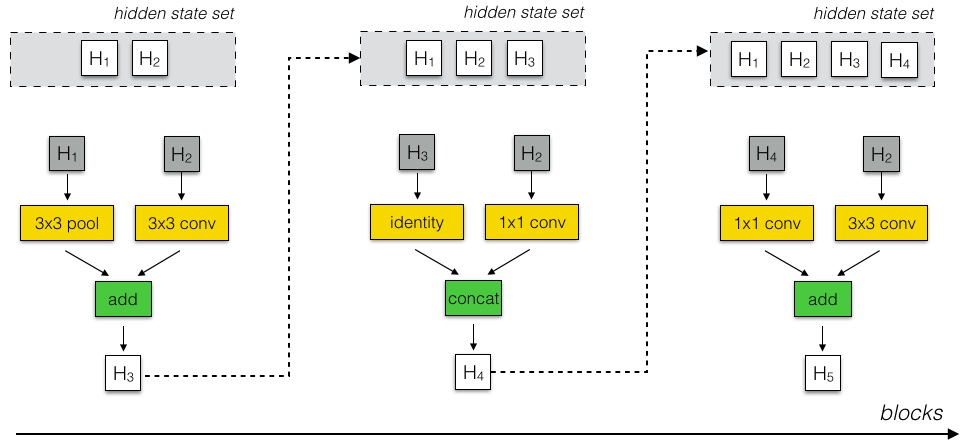
\includegraphics[width=1.9\columnwidth]{NAS-Search-Space.jpeg}
\caption{Schematic diagram of the NASNet search space. Network motifs are constructed recursively in stages termed blocks. Each block consists of the controller selecting a pair of hidden states (dark gray), operations to perform on those hidden states (yellow) and a combination operation (green). The resulting hidden state is retained in the set of potential hidden states to be selected on subsequent blocks.}
\label{figure:nas-search-space}
\end{center}
\end{figure*}

We performed preliminary experiments to identify a flexible, expressive search space for neural architectures that learn effectively. Generally, our strategy for preliminary experiments involved small-scale explorations to identify how to run large-scale architecture search.

\begin{itemize}
\item All convolutions employ ReLU nonlinearity. Experiments with ELU nonlinearity \cite{clevert2015fast} showed minimal benefit.
\item To ensure that the shapes always match in convolutional cells, 1x1 convolutions are inserted as necessary.
\item Unlike \cite{howard2017mobilenets}, all depthwise separable convolution do not employ Batch Normalization and/or a ReLU between the depthwise and pointwise operations.
\item All convolutions followed an ordering of ReLU, convolution operation and Batch Normalization following \cite{identity-mappings}.
\item Whenever a separable convolution is selected as an operation by the model architecture, the separable convolution is applied twice to the hidden state. We found this empirically to improve overall performance.
\end{itemize}


% CONVERT TO DOS AS OPPOSED NOT NOT DOS. - shlens
%We first highlight several negative results that did not lead did to performance gains:

%\begin{itemize}
%\item {\bf Separable convolutions.} Inserting Batch Normalization and/or a ReLU between depthwise and pointwise operations \cite{howard2017mobilenets} in the separable convolution operations.
%\item {\bf Nonlinearities.} Employing ELU \cite{clevert2015fast} instead of ReLUs nonlinearities.
%\item {\bf Regularizations}. L1 regularization of weights and dropout of individual convolutional filters \cite{srivastava2014dropout}.
%\end{itemize}

%We found that adding Batch Normalization and/or a ReLU between the depthwise and pointwise operations in the separable convolution operations to not help performance. L1 regularization was tried with the NASNet models, but this was found to hurt performance. We also tried ELU \cite{clevert2015fast} instead of ReLUs and found that performance was about the same. Dropout ~\cite{srivastava2014dropout} was also tried on the convolutional filters, but this was found to degrade performance.

%\paragraph{Operation Ordering:} All convolution operations that could be predicted are applied within the convolutional cells in the following order: ReLU, convolution operation, Batch Normalization. We found this order to improve performance over a different ordering: convolution operation, Batch Normalization and ReLU -- inline with findings from other papers \cite{identity-mappings}.

%In order to be sure shapes always match in the convolutional cells, 1x1 convolutions are inserted as necessary. \todo{Specifically, where are they inserted?}

%\paragraph{Cell Path Dropout:} When training our NASNet models, we found stochastically dropping out each path (edge with a yellow box) in the cell with some fixed probability to be an extremely good regularizer. This is similar to \cite{stochastic} and \cite{zhang2016polynet} where they dropout full parts of their model during training and then at test time scale the path by the probability of keeping that path during training. Interestingly we found that linearly increasing the probability of dropping out a path over the course of training to significantly improve the final performance for both CIFAR and ImageNet experiments.

\subsection{Training with ScheduledDropPath}
We performed several experiments with various stochastic regularization methods. Naively applying dropout \cite{srivastava2014dropout} across convolutional filters degraded performance. However,  we discovered a new technique called \emph{ScheduledDropPath}, a modified version of DropPath~\cite{larsson2016fractalnet}, that works well in regularizing NASNets. In DropPath, we stochastically drop out each path (i.e., edge with a yellow box in Figure \ref{figure:cell_structure}) in the cell with some fixed probability. This is similar to \cite{stochastic} and \cite{zhang2016polynet} where they dropout full parts of their model during training and then at test time scale the path by the probability of keeping that path during training. Interestingly we also found that DropPath alone does not help NASNet training much, but DropPath with \emph{linearly increasing the probability of dropping out a path over the course of training}  significantly improves the final performance for both CIFAR and ImageNet experiments. We name this method ScheduledDropPath.

\subsection{Training of CIFAR models}
All of our CIFAR models use a single period cosine decay as in \cite{loshchilov2016sgdr, gastaldi17shakeshake}.  All models use the momentum optimizer with momentum rate set to 0.9. All models also use L2 weight decay. Each architecture is trained for a fixed 20 epochs on CIFAR-10 during the architecture search process. Additionally, we found it beneficial to use the cosine learning rate decay during the 20 epochs the CIFAR models were trained as this helped to further differentiate good architectures. We also found that having the CIFAR models use a small $N=2$ during the architecture search process allowed for models to train quite quickly, while still finding cells that work well once more were stacked.

\subsection{Training of ImageNet models}

We use ImageNet 2012 ILSVRC challenge data for large scale image classification. The dataset consists of $\sim$ 1.2M images labeled across 1,000 classes \cite{deng2009imagenet}. Overall our training and testing procedures are almost identical to \cite{szegedy2016rethinking}. ImageNet models are trained and evaluated on 299x299 or 331x331 images using the same data augmentation procedures as described previously \cite{szegedy2016rethinking}. We use distributed synchronous SGD to train the ImageNet model with 50 workers (and 3 backup workers) each with a Tesla K40 GPU \cite{synchsgd}. We use RMSProp with a decay of 0.9 and epsilon of 1.0. Evaluations are calculated using with a running average of parameters over time with a decay rate of 0.9999. We use label smoothing with a value of 0.1 for all ImageNet models as done in \cite{szegedy2016rethinking}. Additionally, all models use an auxiliary classifier located at 2/3 of the way up the network. The loss of the auxiliary classifier is weighted by 0.4 as done in \cite{szegedy2016rethinking}. We empirically found our network to be insensitive to the number of parameters associated with this auxiliary classifier along with the weight associated with the loss. All models also use L2 regularization.  The learning rate decay scheme is the exponential decay scheme used in \cite{szegedy2016rethinking}.  Dropout is applied to the final softmax matrix with probability 0.5.




%\fi


\section{Additional Experiments}
\label{sec:othernasnet}
We now present two additional cells that performed well on CIFAR and ImageNet. The search spaces used for these cells are slightly different than what was used for NASNet-A. For the NASNet-B model in Figure \ref{figure:cell_structure_b} we do not concatenate all of the unused hidden states generated in the convolutional cell. Instead all of the hiddenstates created within the convolutional cell, even if they are currently used, are fed into the next layer. Note that $B=4$ and there are 4 hiddenstates as input to the cell as these numbers must match for this cell to be valid. We also allow addition followed by layer normalization \cite{ba2016layer} or instance normalization \cite{ulyanov2016instance} to be predicted as two of the combination operations within the cell, along with addition or concatenation. 


\begin{figure}[h!]
\begin{center}
%\includegraphics[width=0.58\columnwidth]{figures/Barret_cell1.eps}
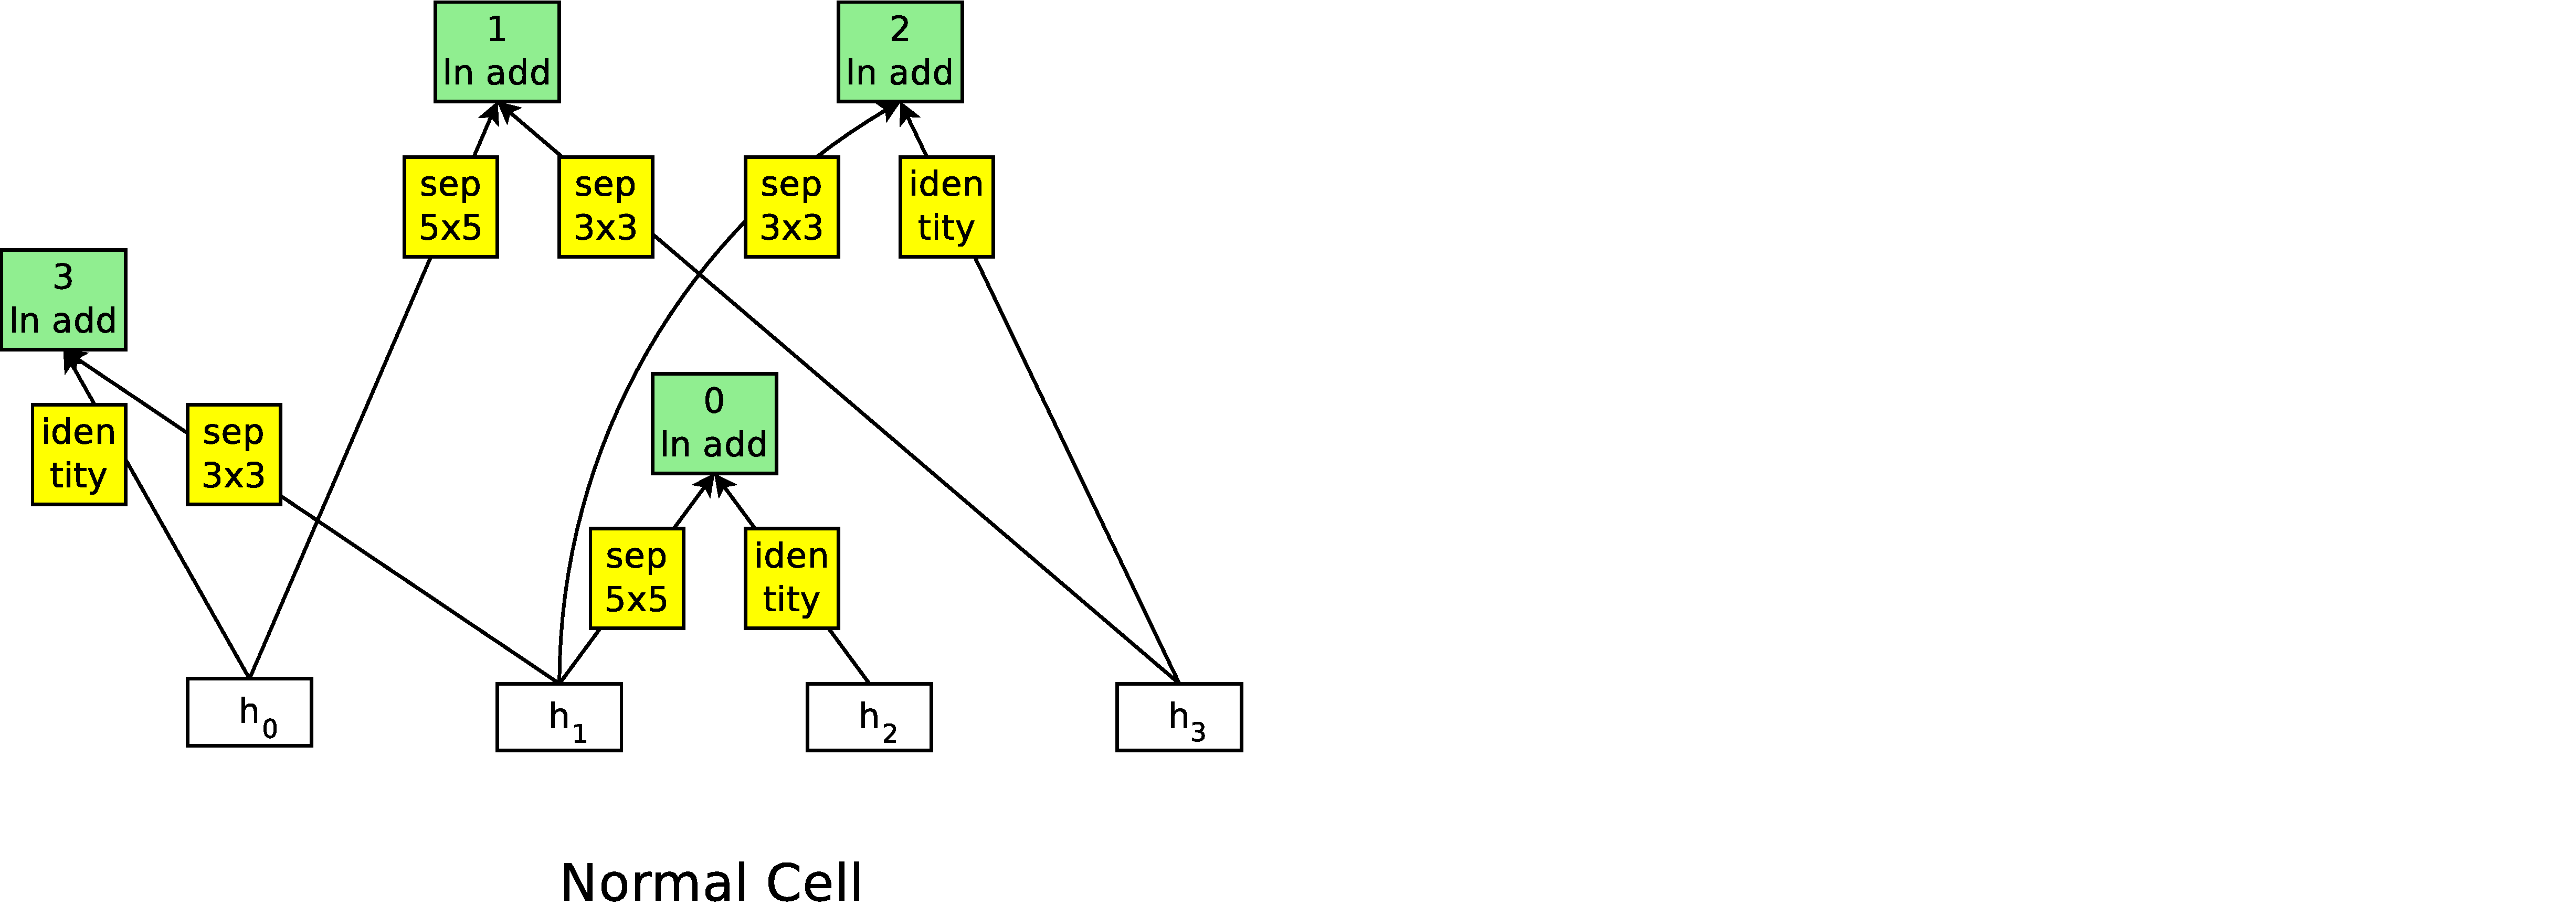
\includegraphics[width=\columnwidth]{Cell-B-Normal.pdf} \\
\vspace{0.4cm}
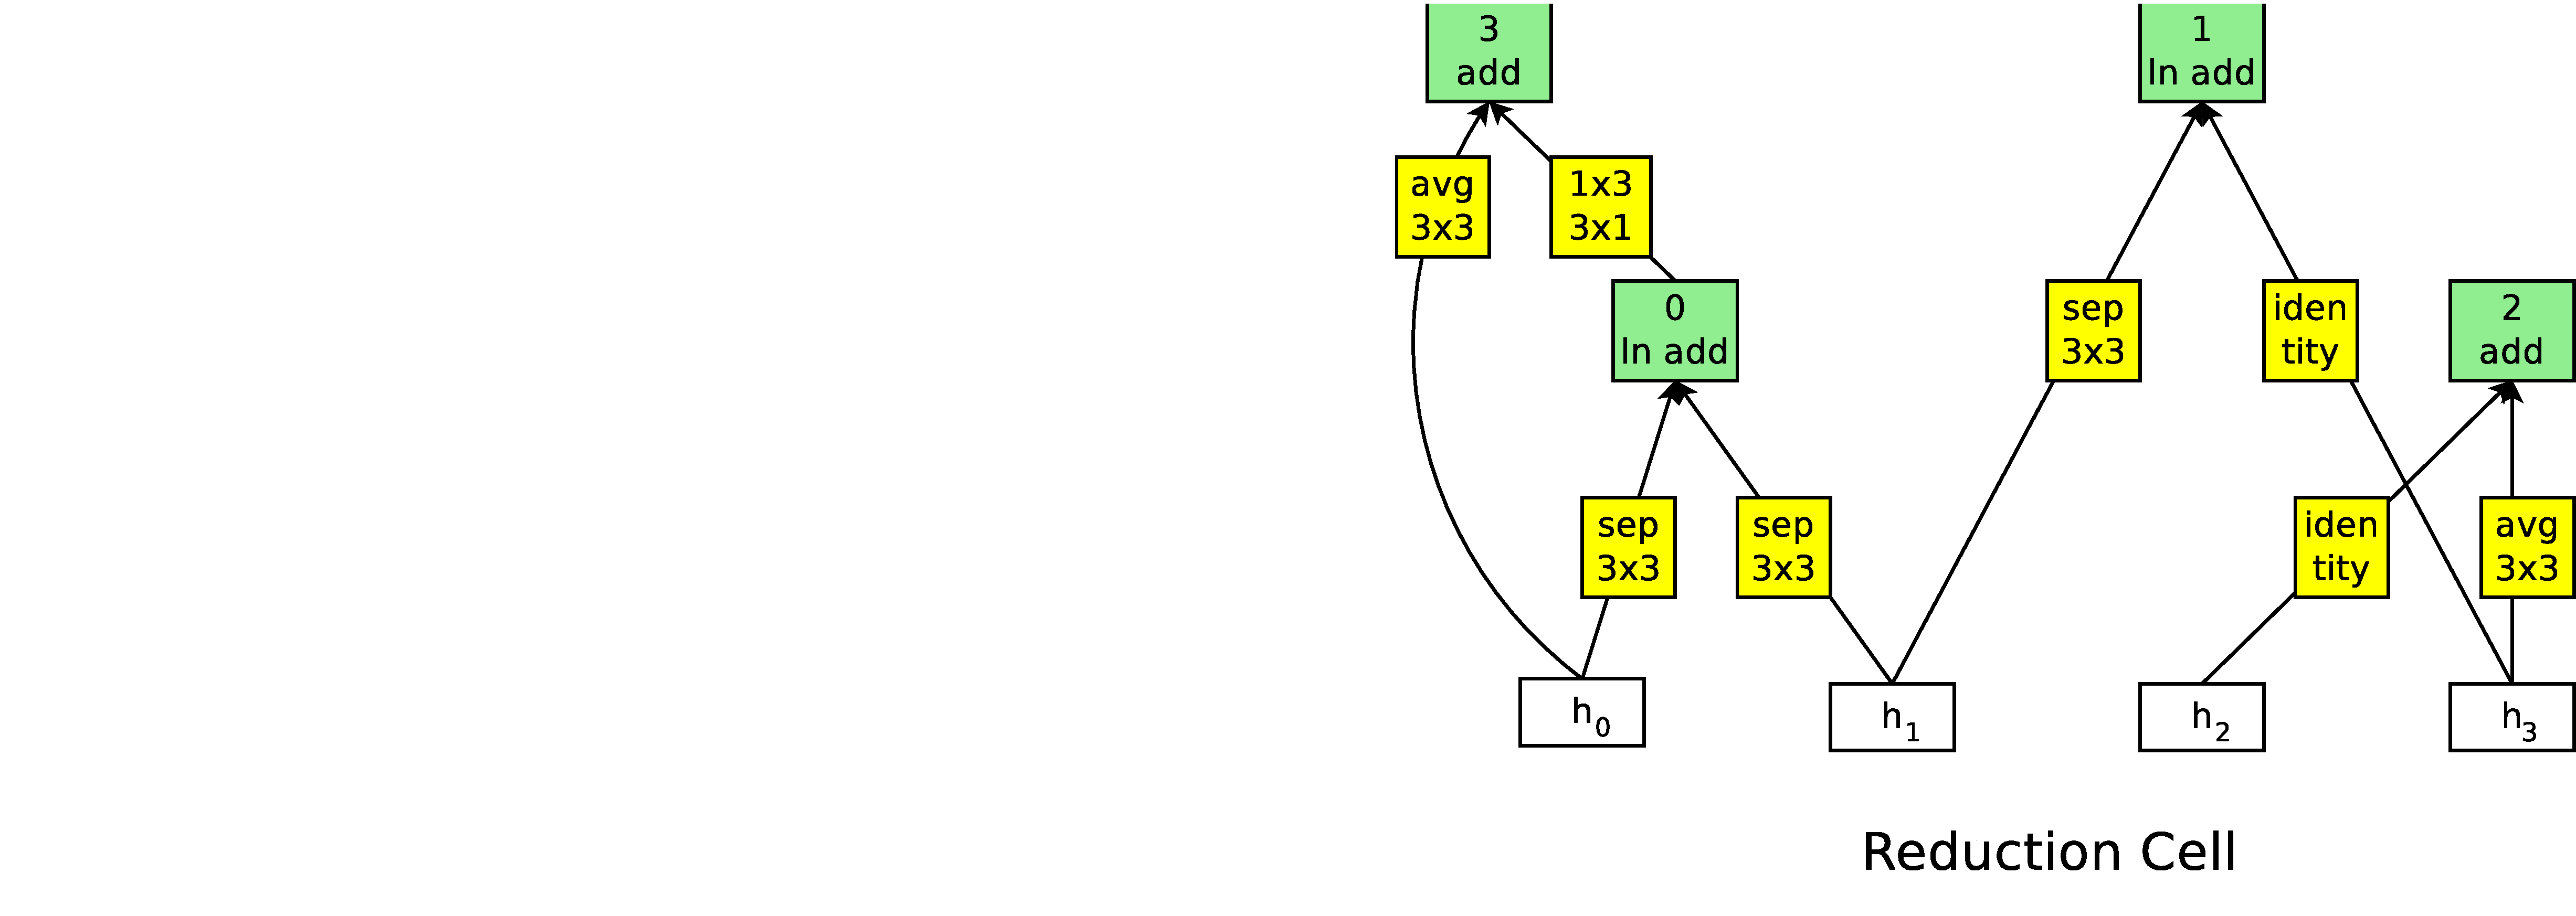
\includegraphics[width=\columnwidth]{Cell-B-Reduction.pdf}
\caption{Architecture of NASNet-B convolutional cell with $B=4$ blocks identified with CIFAR-10. The input (white) is the hidden state from previous activations (or input image).
Each convolutional cell is the result of $B$ blocks.
A single block is corresponds to two primitive operations (yellow) and a combination operation (green). As do we not concatenate the output hidden states, each output hidden state is used as a hidden state in the future layers. Each cell takes in 4 hidden states and thus needs to also create 4 output hidden states. Each output hidden state is therefore labeled with 0, 1, 2, 3 to represent the next four layers in that order.
%Left is the Normal Cell and right is the Reduction Cell.
}
\label{figure:cell_structure_b}
\end{center}
\end{figure}

\begin{figure}[h!]
\begin{center}
%\includegraphics[width=0.58\columnwidth]{figures/Barret_cell1.eps}
%\includegraphics[width=0.9\linewidth]{figures/CellC.eps}
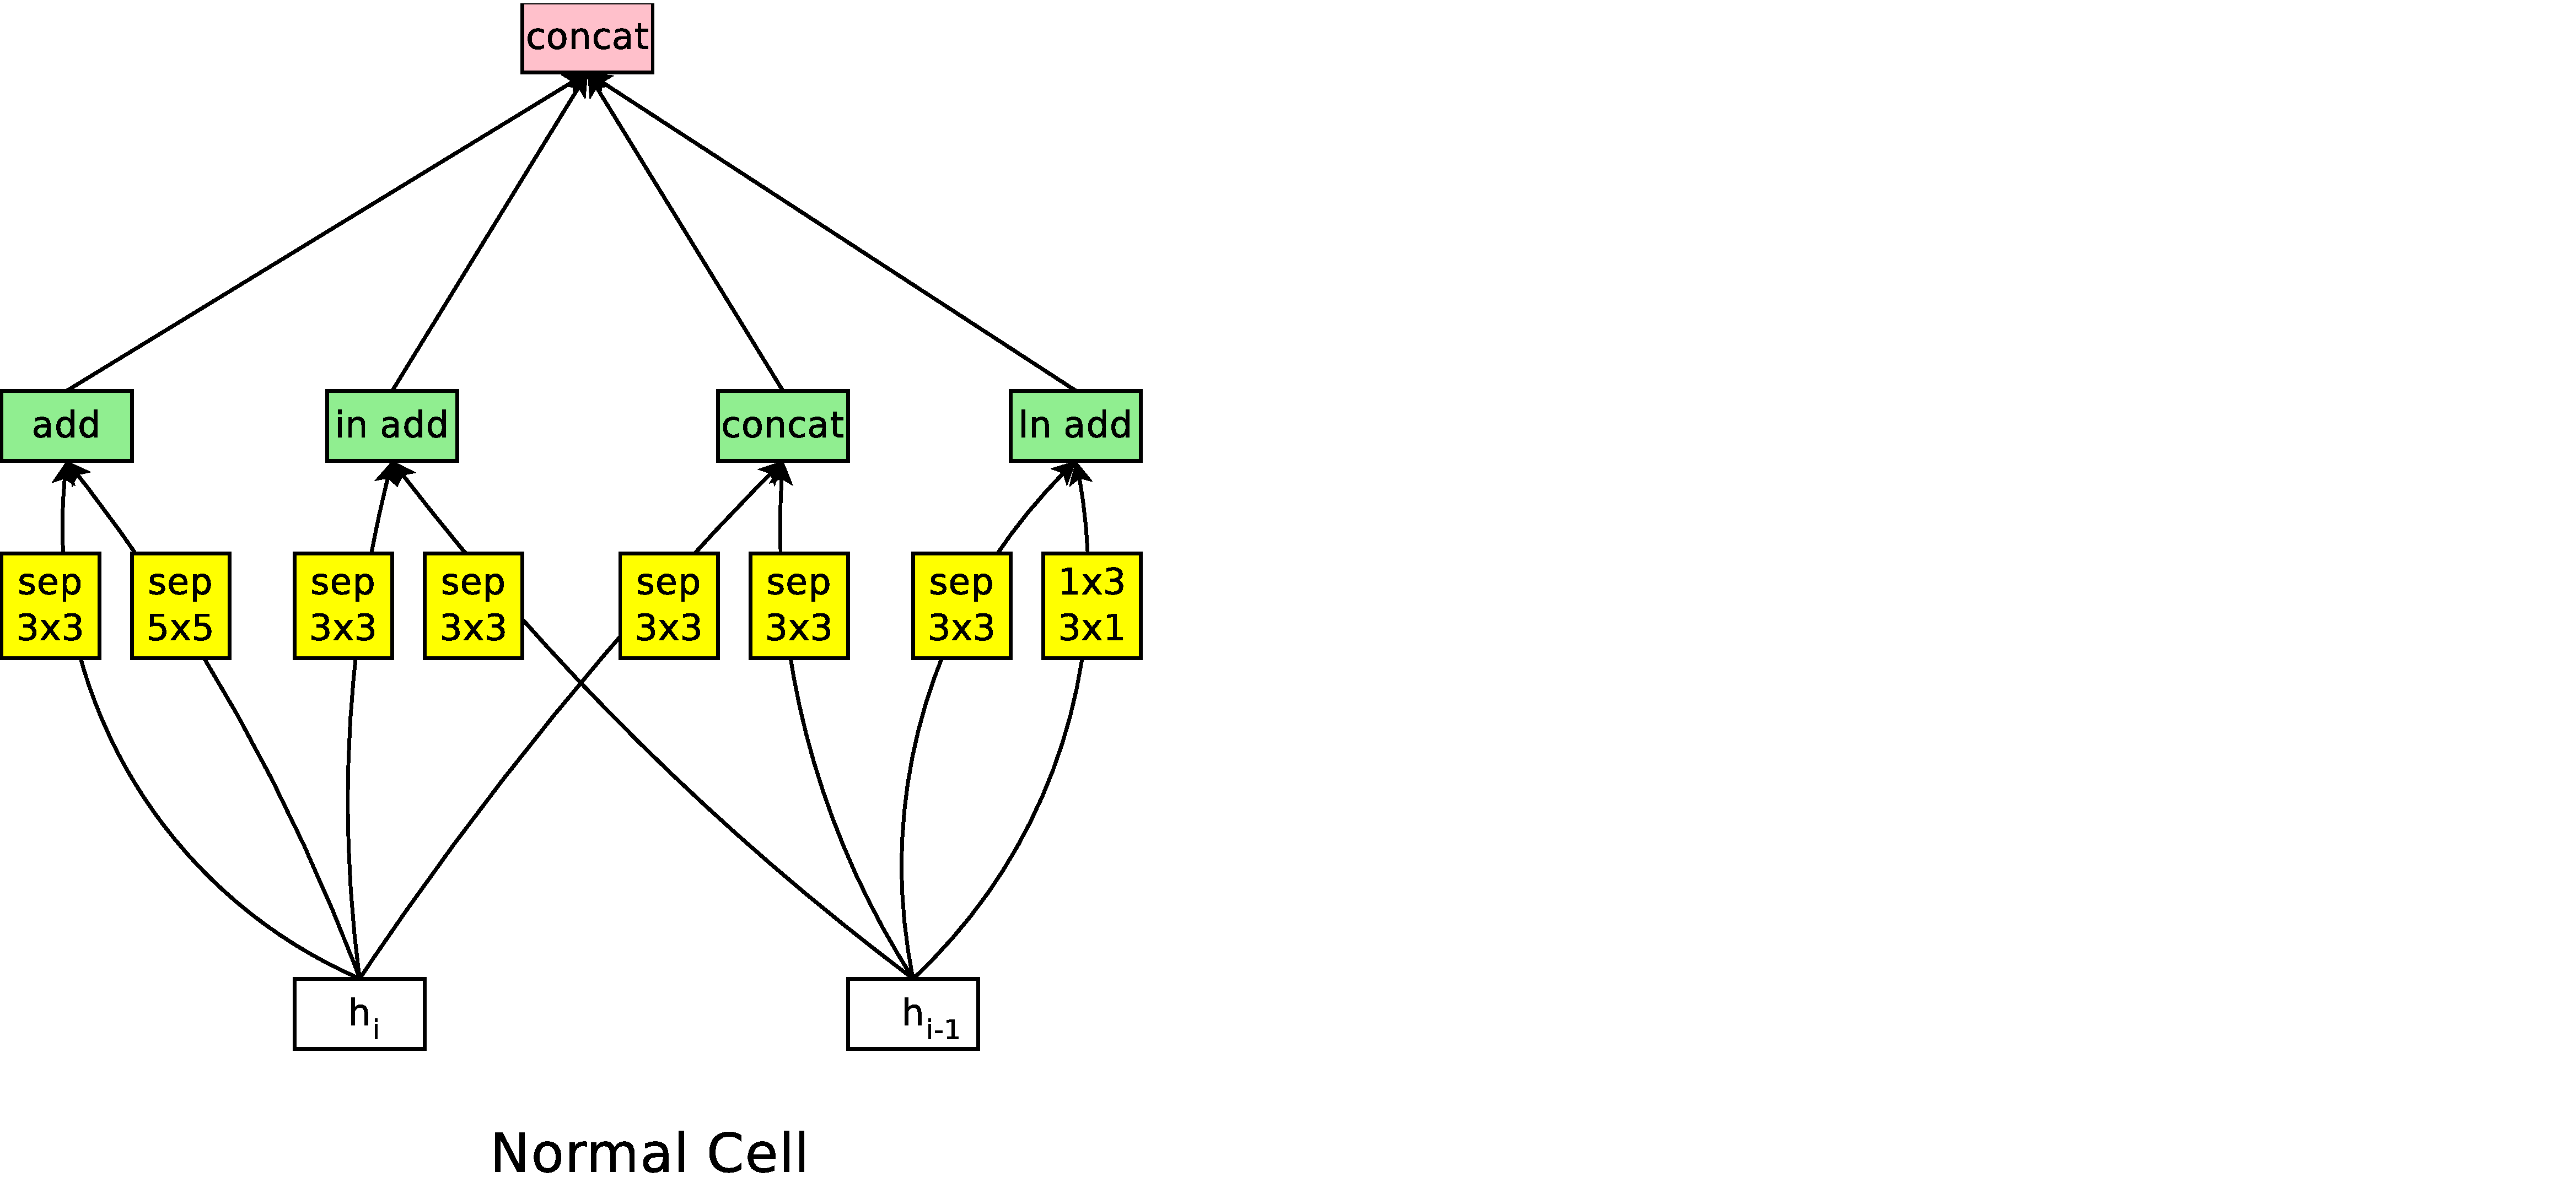
\includegraphics[width=\columnwidth]{Cell-C-Normal.pdf} \\
\vspace{0.4cm}
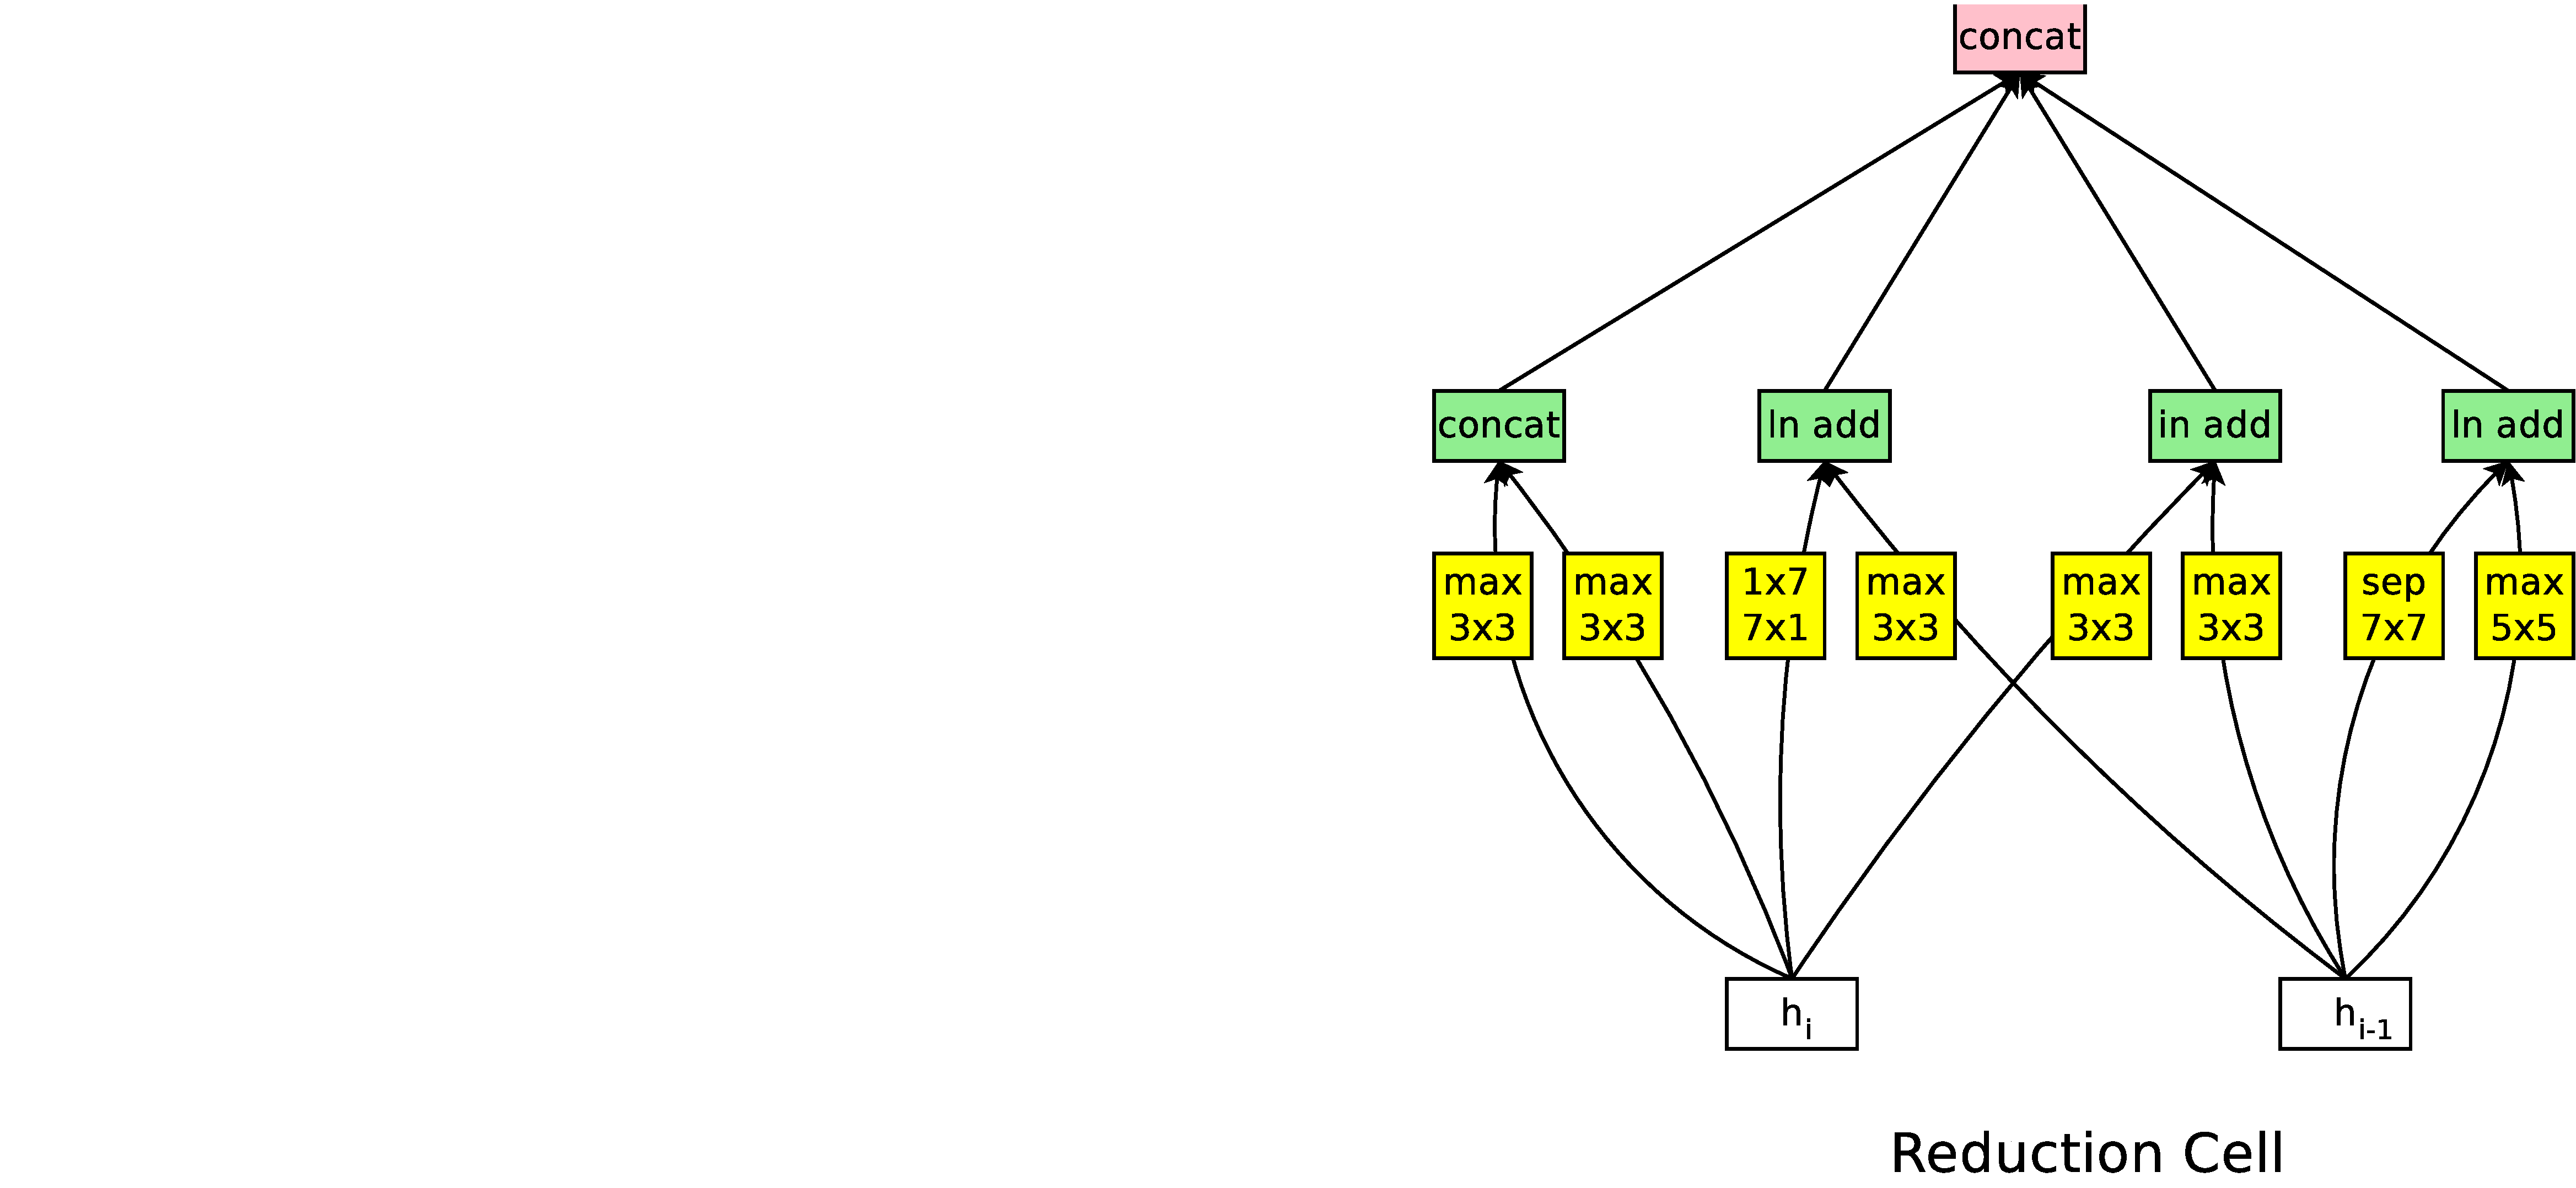
\includegraphics[width=\columnwidth]{Cell-C-Reduction.pdf}
\caption{Architecture of NASNet-C convolutional cell with $B=4$ blocks identified with CIFAR-10. The input (white) is the hidden state from previous activations (or input image). The output (pink) is the result of a concatenation operation across all resulting branches.
Each convolutional cell is the result of $B$ blocks.
A single block corresponds to two primitive operations (yellow) and a combination operation (green). 
%Left is the Normal Cell and right is the Reduction Cell.
}
\label{figure:cell_structure_c}
\end{center}
\end{figure}

For NASNet-C (Figure~\ref{figure:cell_structure_c}), we concatenate all of the unused hidden states generated in the convolutional cell like in NASNet-A, but now we allow the prediction of addition followed by layer normalization or instance normalization like in NASNet-B.


\section{Example object detection results}
\label{sec:object_detection}
Finally, we will present examples of object detection results on the COCO dataset in  Figure~\ref{figure:object-detection} and Figure~\ref{figure:object-detection-examples}. As can be seen from the figures, NASNet-A featurization works well with Faster-RCNN and gives accurate localization of objects.

\iffalse
\begin{figure}[h!]
\begin{center}
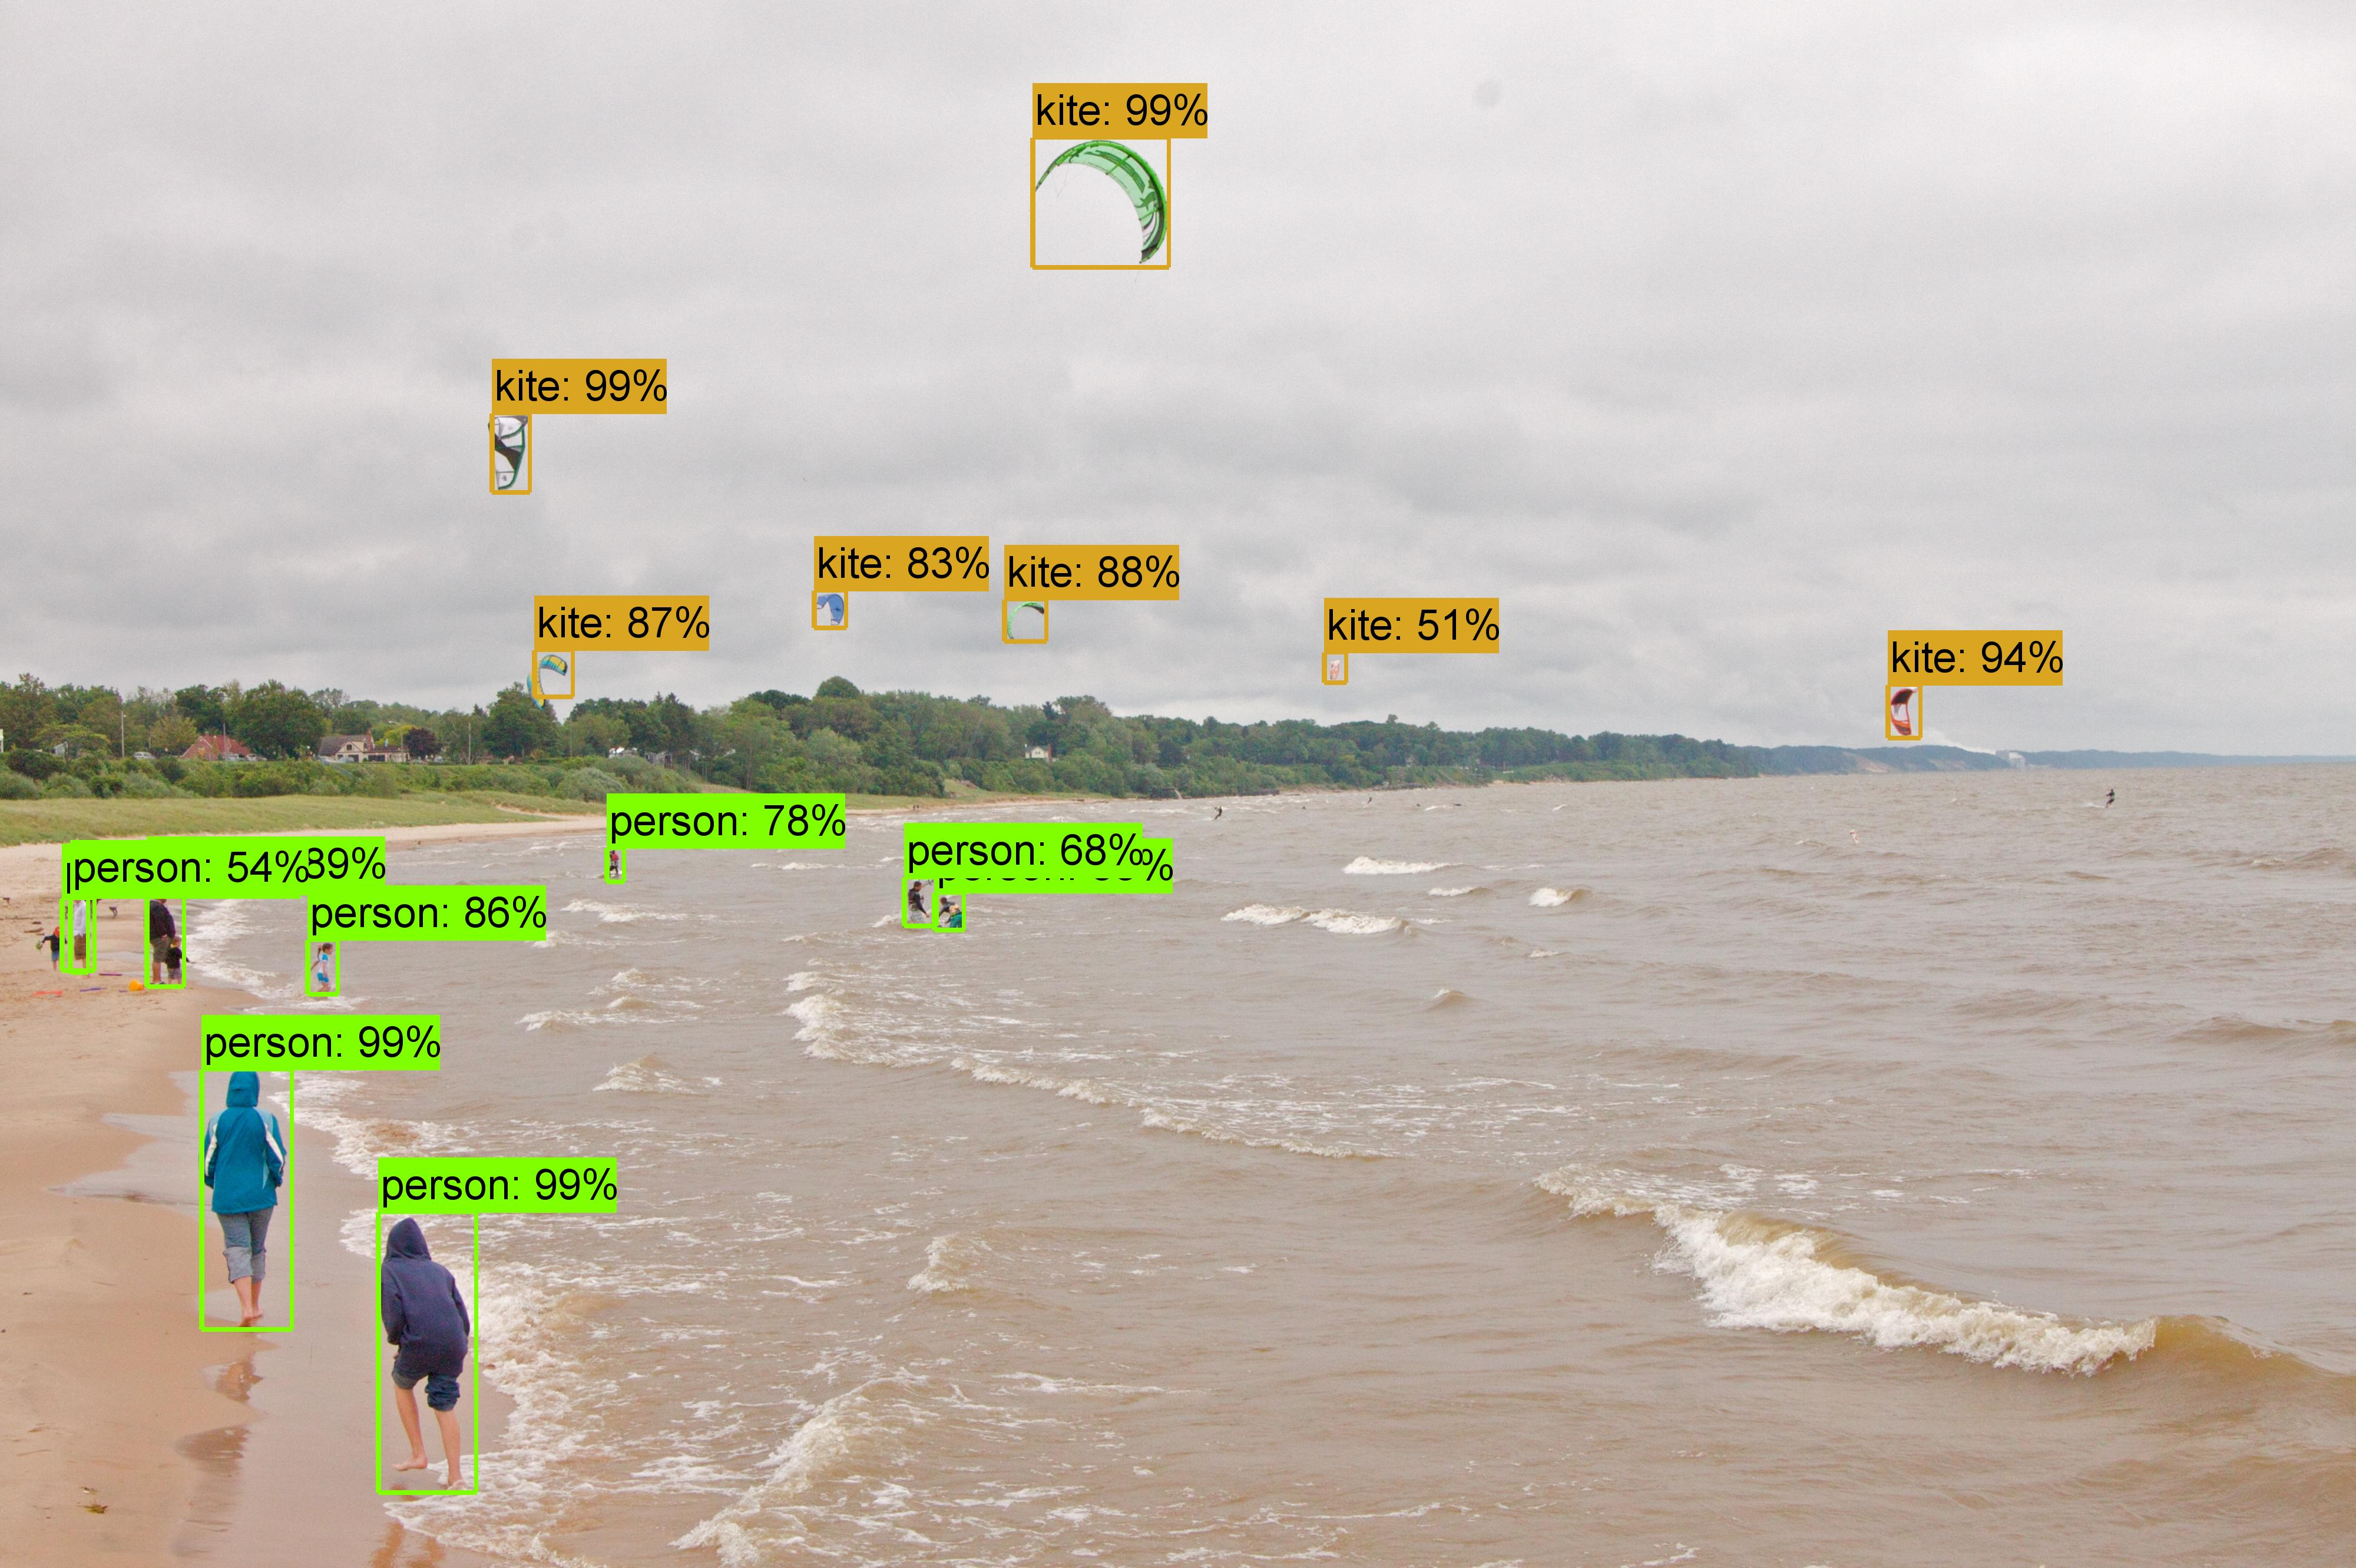
\includegraphics[width=\columnwidth]{Kite-Surf-Inception-ResNet-v2.jpg}
\hfill
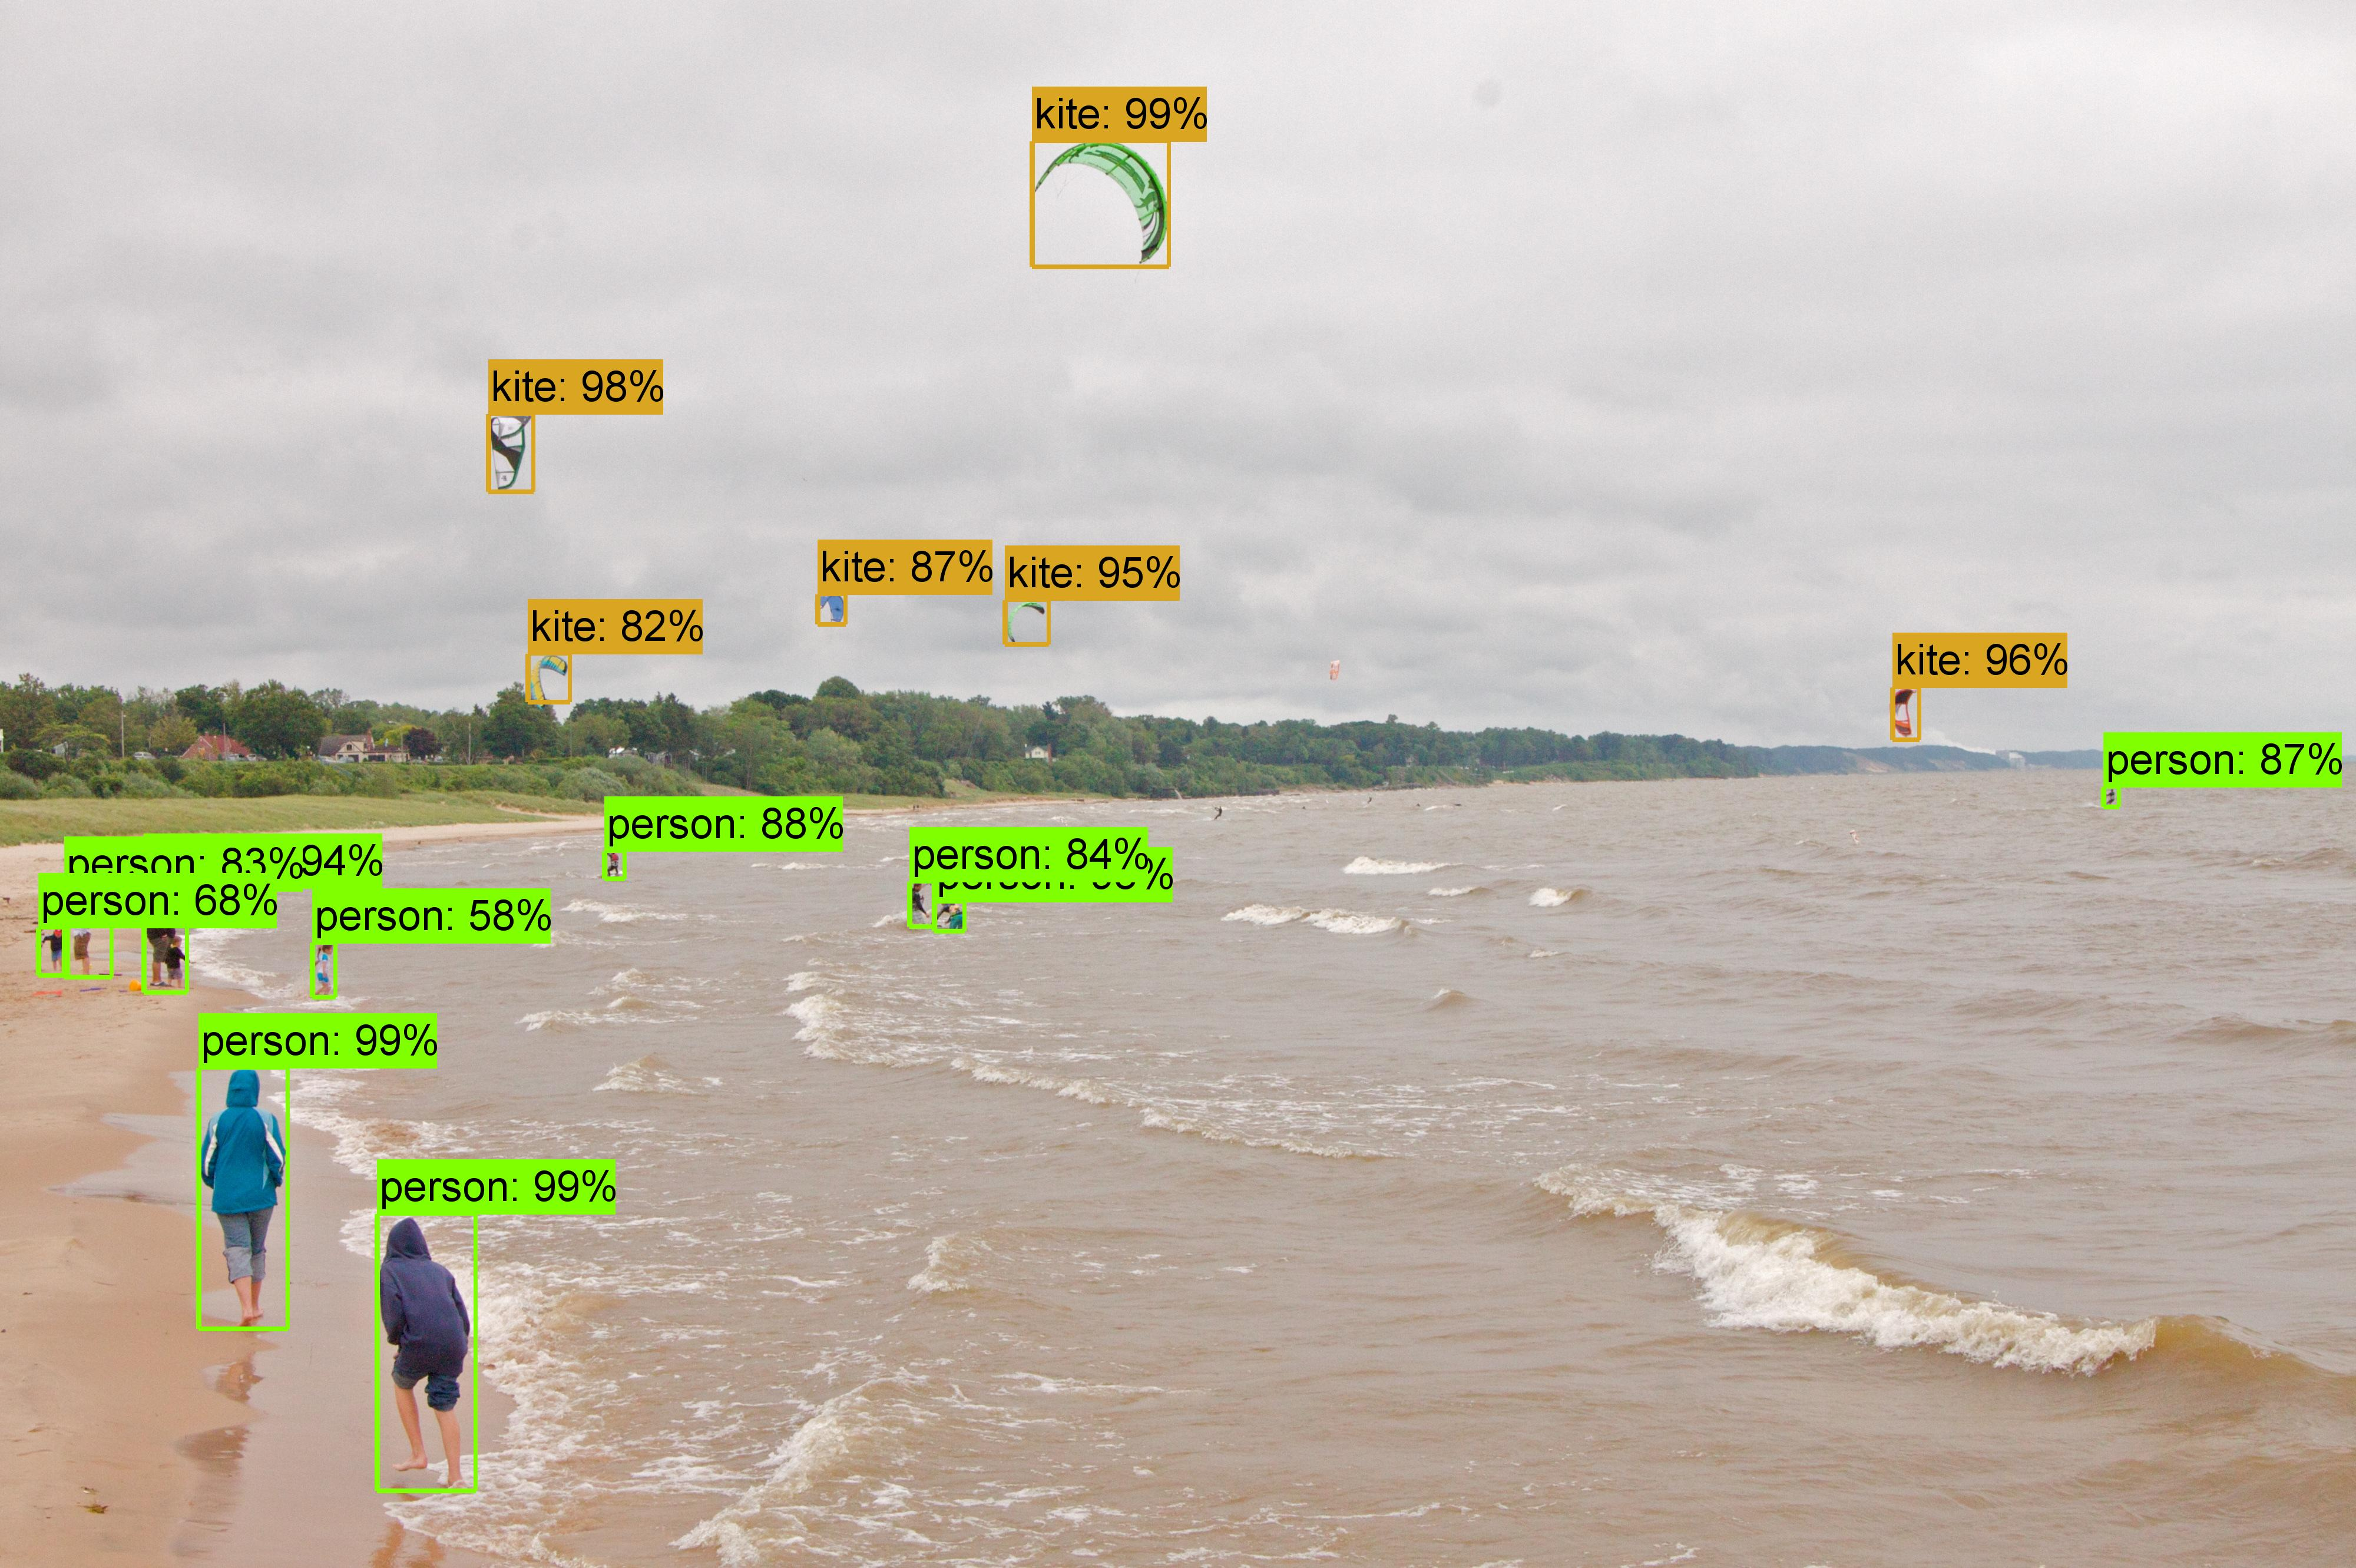
\includegraphics[width=\columnwidth]{Kite-Surf-NAS.jpg}
\caption{Example detections showcasing improvements of object detection over previous state-of-the-art model for Faster-RCNN with Inception-ResNet-v2 featurization \cite{huang2016speed} (top)
and NASNet-A featurization (bottom).
}
\label{figure:object-detection}
\end{center}
\end{figure}
\fi



\begin{figure}[h!]
\begin{center}
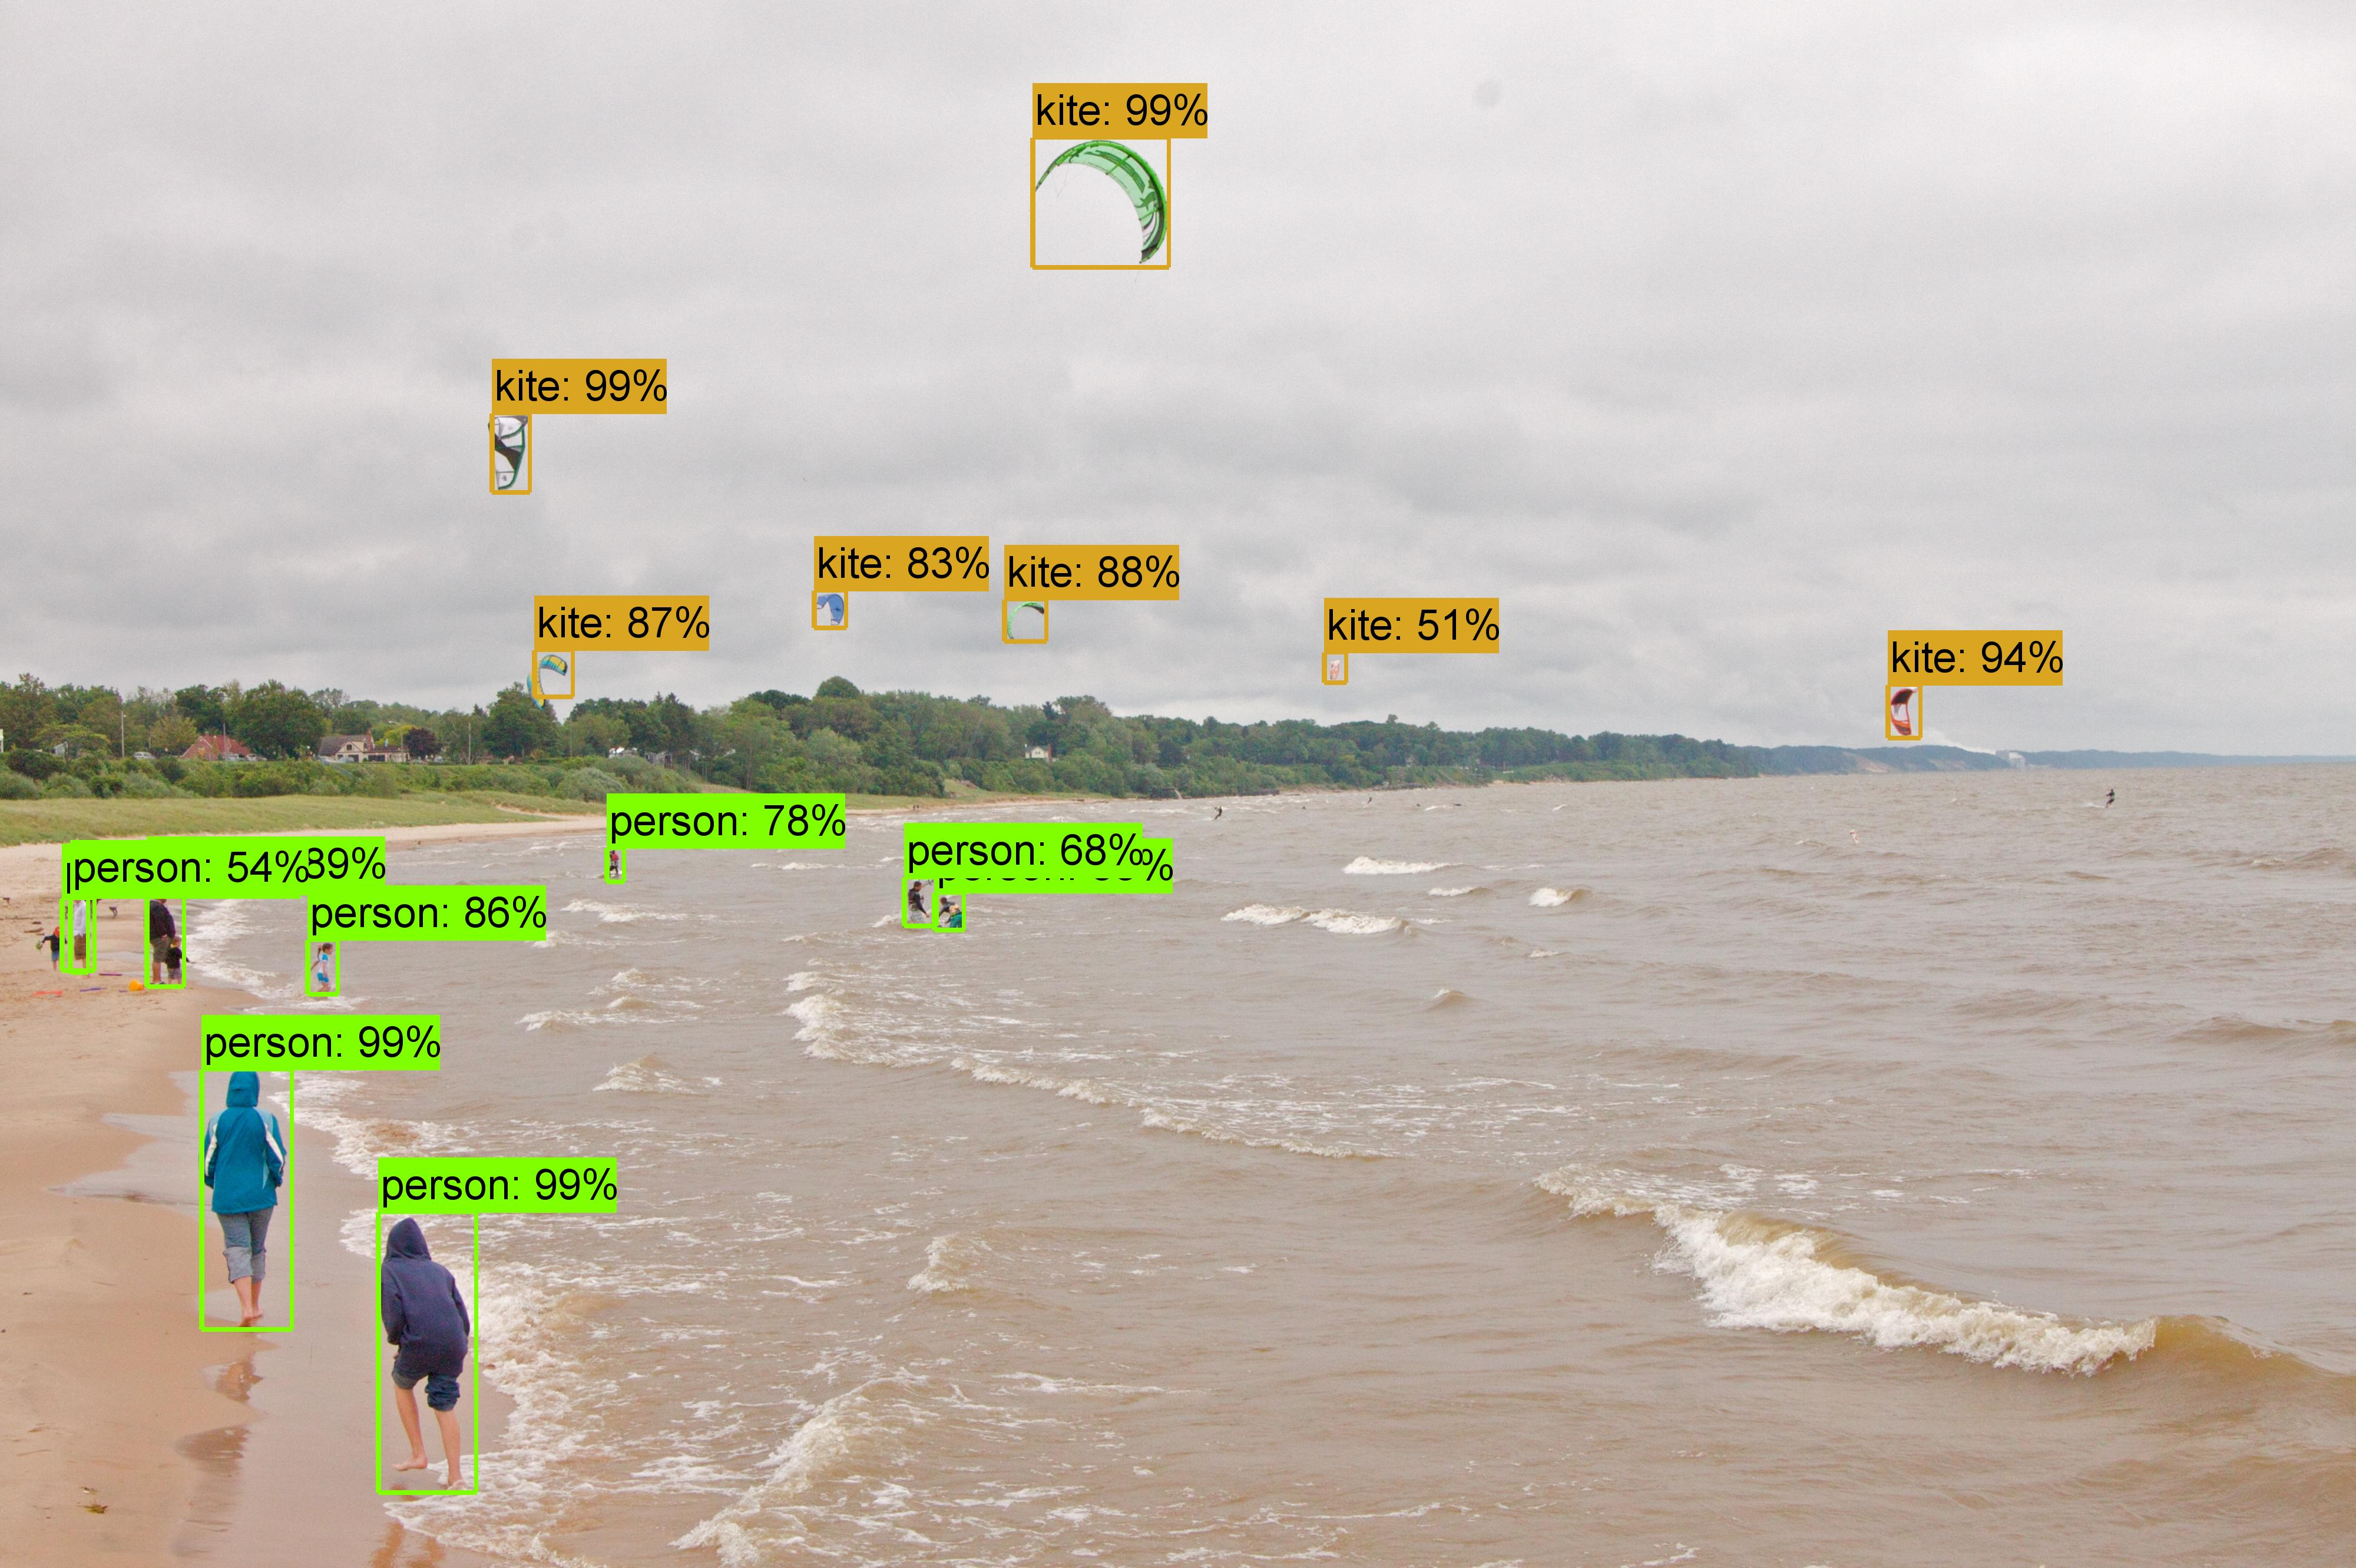
\includegraphics[width=0.98\columnwidth]{Kite-Surf-Inception-ResNet-v2.jpg}
\hfill
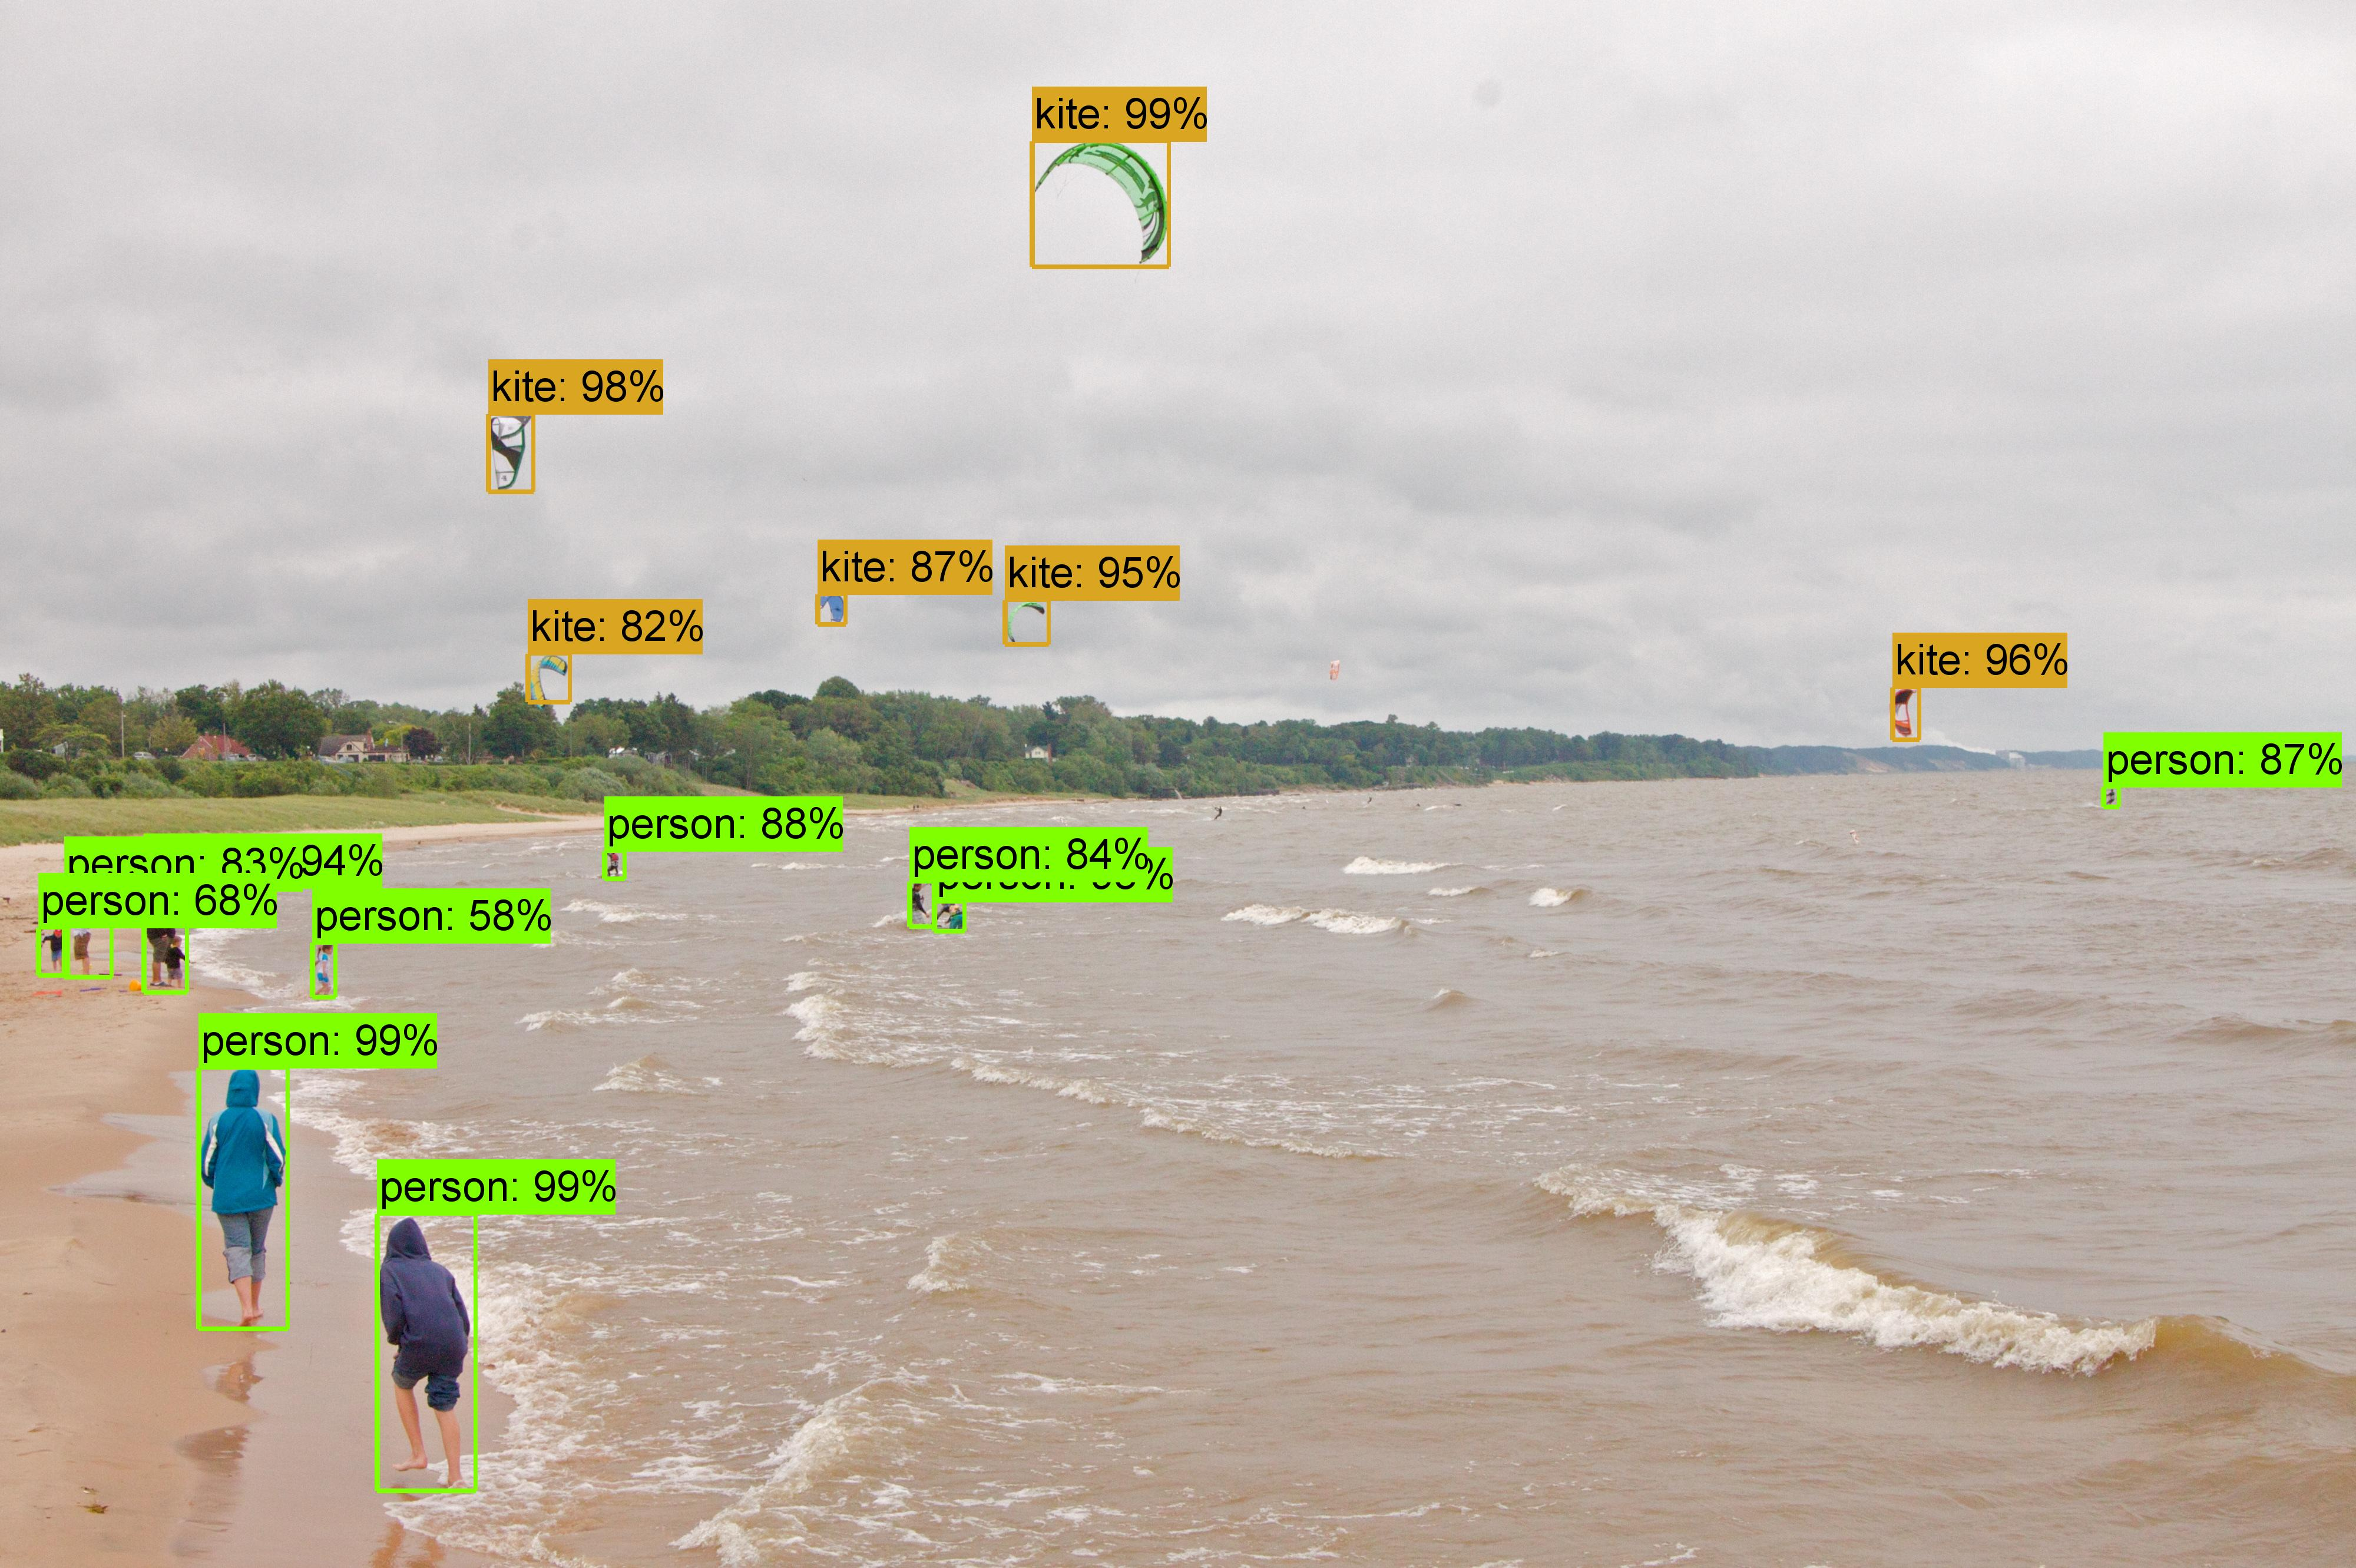
\includegraphics[width=0.98\columnwidth]{Kite-Surf-NAS.jpg}
\caption{Example detections showing improvements of object detection over previous state-of-the-art model for Faster-RCNN with Inception-ResNet-v2 featurization \cite{huang2016speed} (top)
and NASNet-A featurization (bottom). %Notice that NASNet-A succeeds in detecting a small person on the right side of the image.
}
\label{figure:object-detection}
\end{center}
\end{figure}

\begin{figure}[h!]
\begin{center}
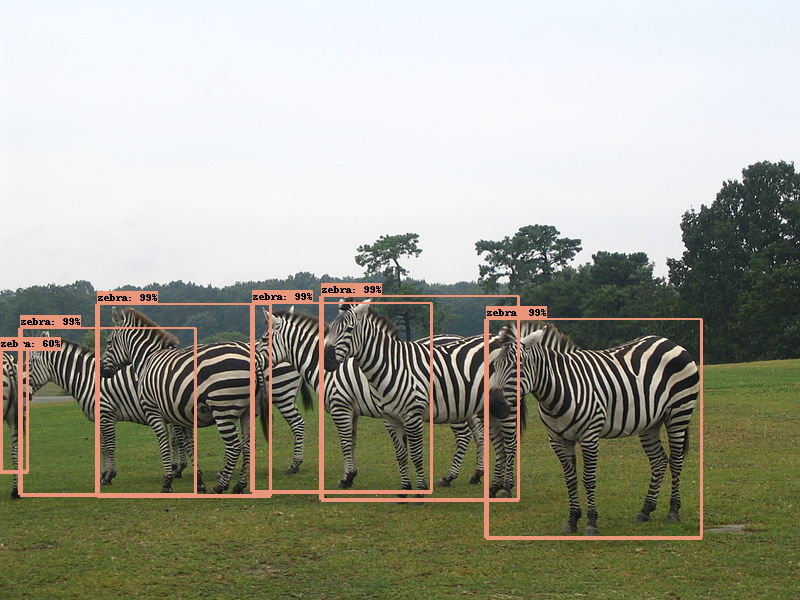
\includegraphics[width=\columnwidth]{Detection-Zebras.png}
\hfill
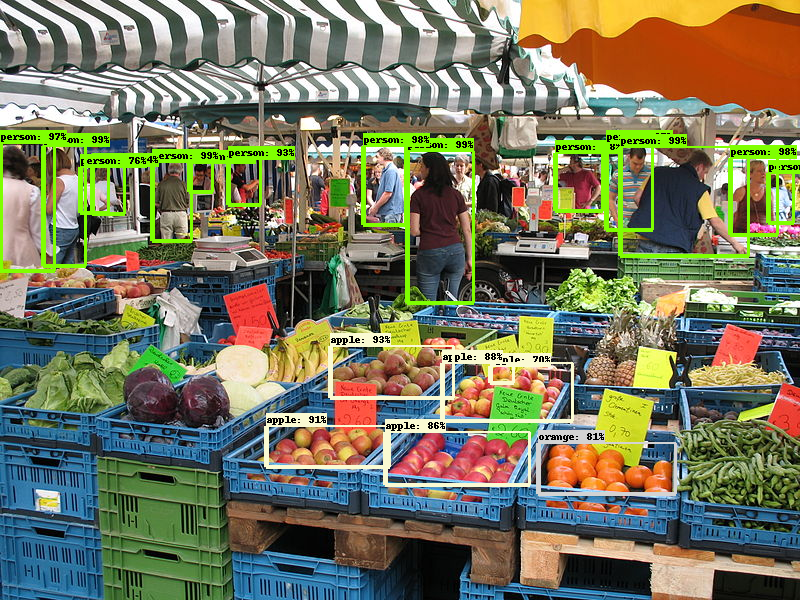
\includegraphics[width=\columnwidth]{Detection-Market.png}
\hfill
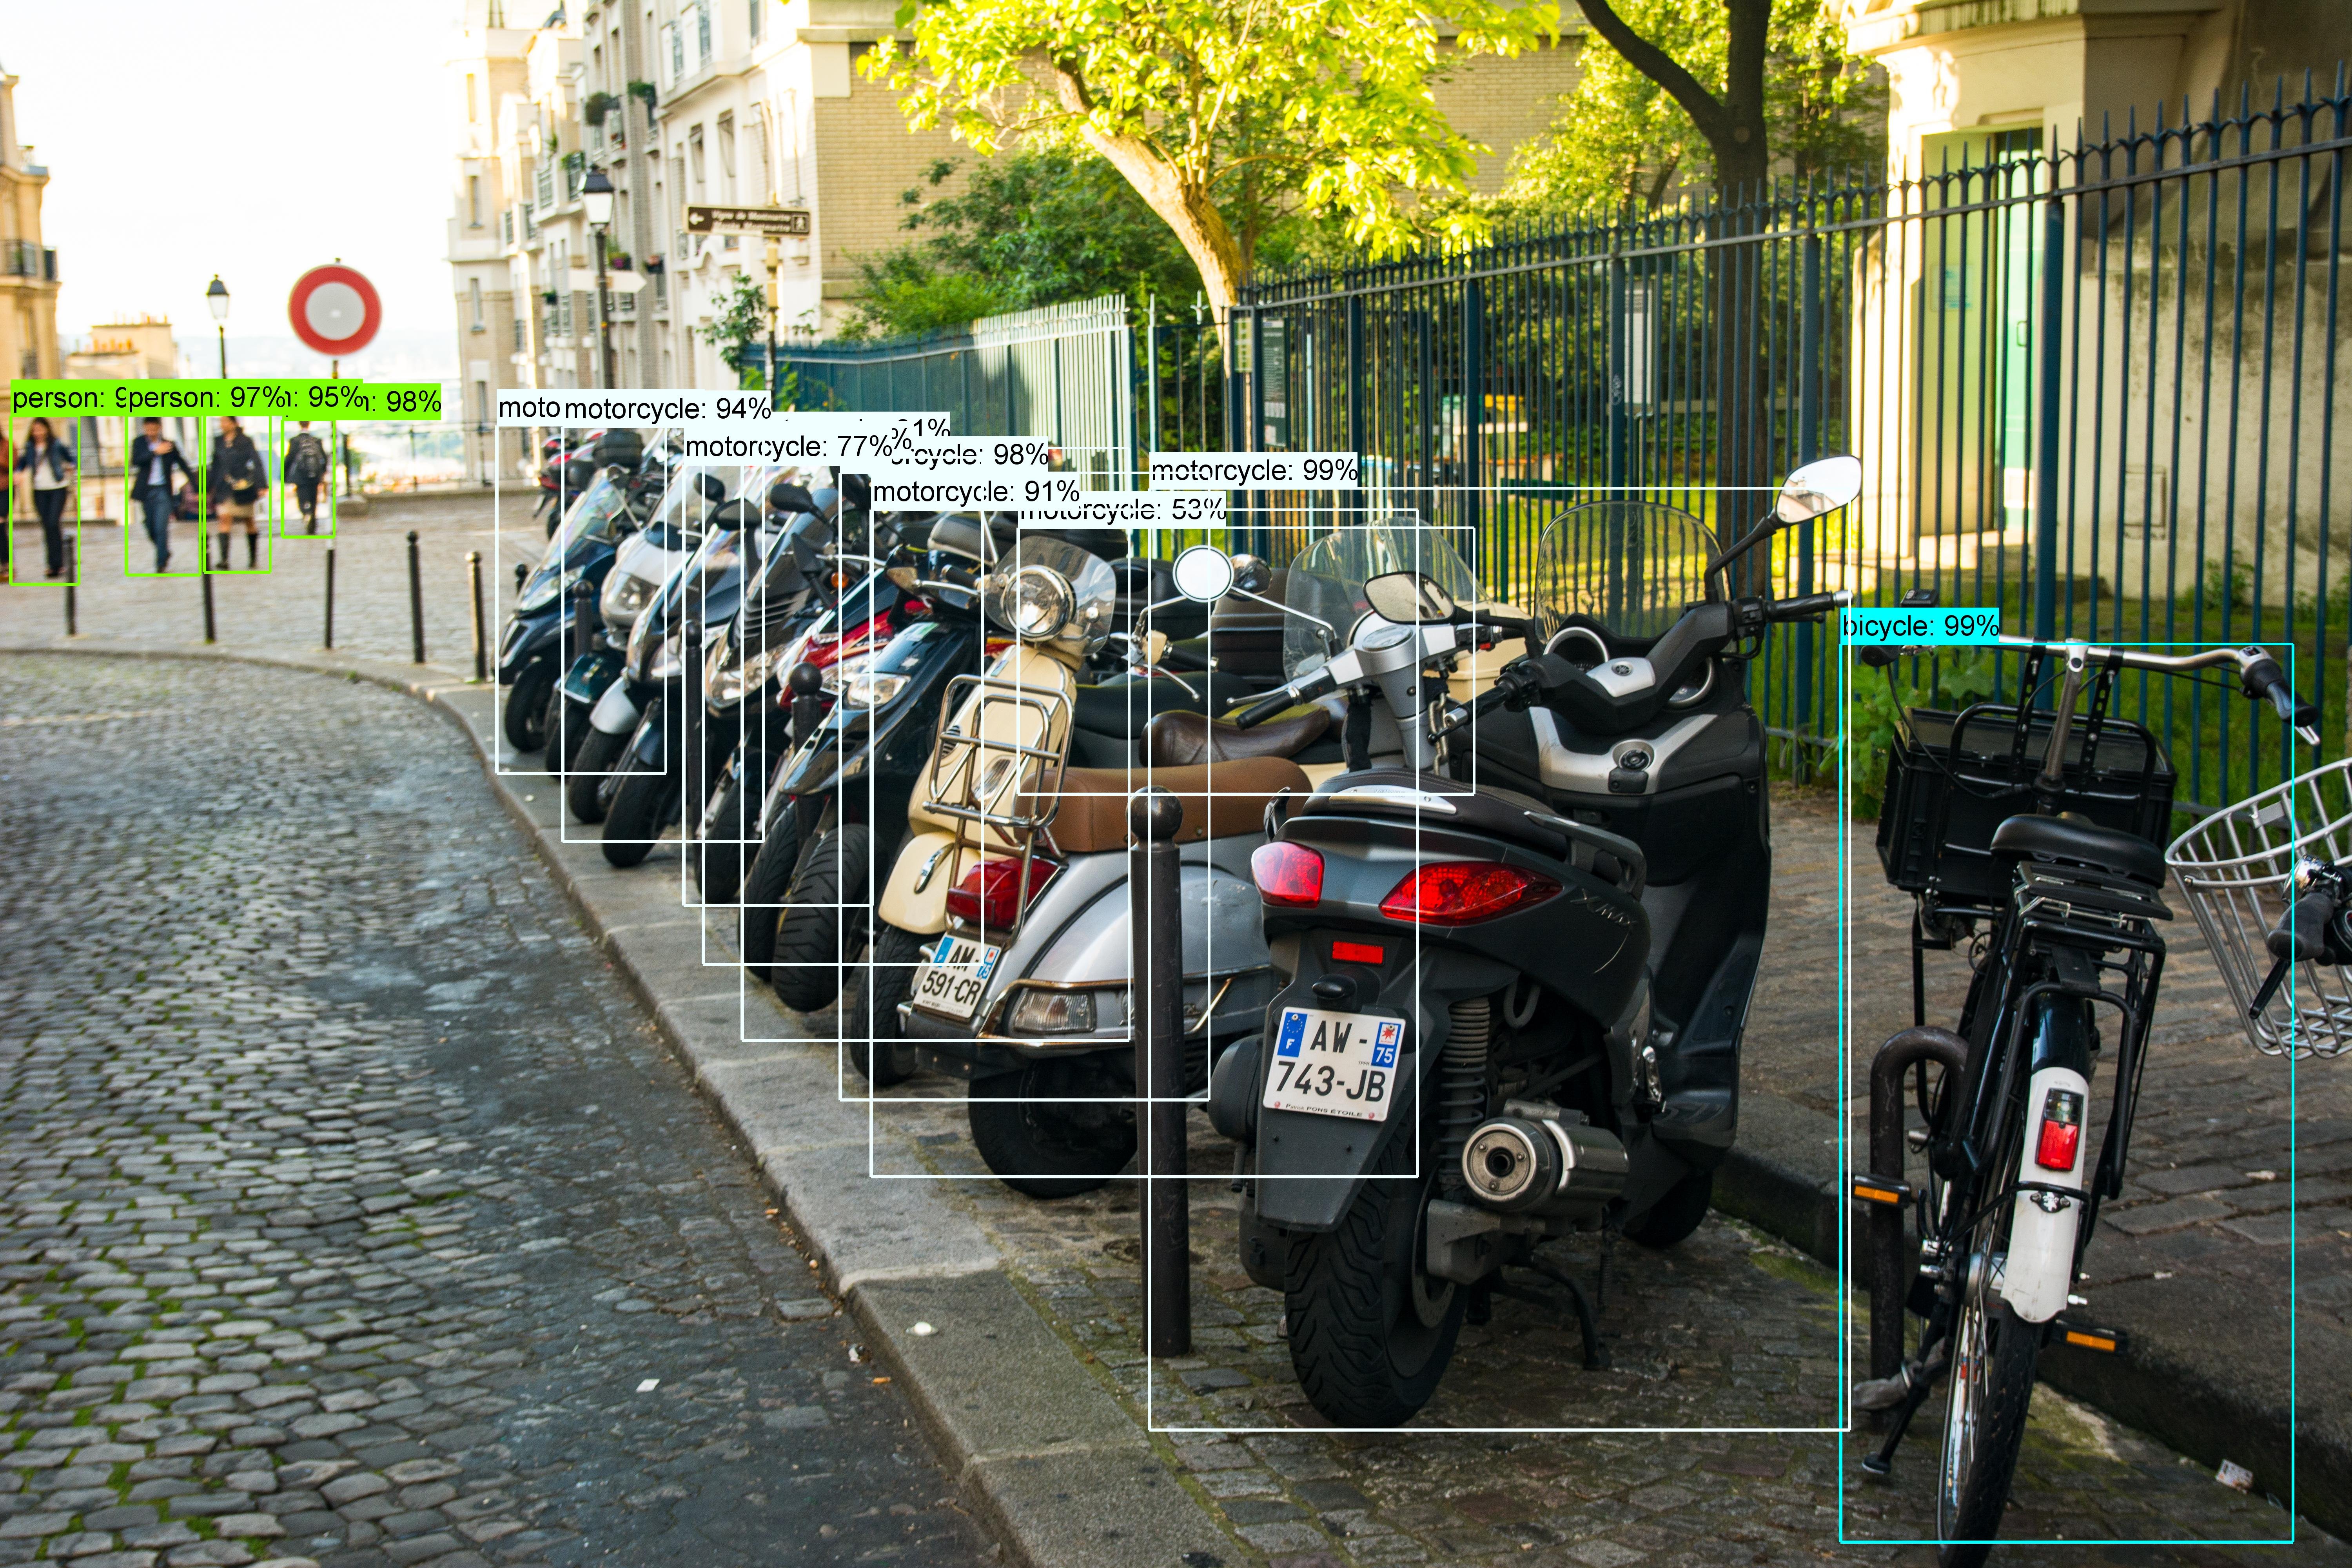
\includegraphics[width=\columnwidth]{Detection-Moped.jpeg}
\caption{Example detections of best performing NASNet-A featurization with Faster-RCNN trained on COCO dataset. Top and middle images courtesy of \texttt{http://wikipedia.org}. Bottom image courtesy of Jonathan Huang}
\label{figure:object-detection-examples}
\end{center}
\end{figure}
